%!TEX encoding = UTF-8 Unicode
\documentclass{beamer}
\usetheme{Copenhagen}
\usecolortheme{default}

% beamer settings
\setbeamertemplate{right corner}
{\insertshortdate{}\hspace*{2em}
\insertframenumber{} / \inserttotalframenumber}
\makeatletter
\setbeamertemplate{footline}
{\leavevmode%
\hbox{%

% right colorbox
\begin{beamercolorbox}[wd=.333333\paperwidth,ht=2.25ex,dp=1ex,center]
{author in head/foot}%
\usebeamerfont{author in head/foot}\insertshortauthor\expandafter\beamer@ifempty\expandafter{\beamer@shortinstitute}{}{~~(\insertshortinstitute)}
\end{beamercolorbox}%

% center colorbox
\begin{beamercolorbox}[wd=.333333\paperwidth,ht=2.25ex,dp=1ex,center]
{title in head/foot}%
\usebeamerfont{title in head/foot}\insertshorttitle
\end{beamercolorbox}%

% left colorbox
\begin{beamercolorbox}[wd=.333333\paperwidth,ht=2.25ex,dp=1ex,right]
{date in head/foot}%
\usebeamerfont{date in head/foot}\usebeamertemplate{right corner}\hspace*{2ex} 
\end{beamercolorbox}}%
\vskip0pt}

% packages
\usepackage[utf8]{inputenc}
\usepackage{graphicx}
\usepackage{physics}
\usepackage{booktabs}
\usepackage{subcaption}
\usepackage{subfiles}
\usepackage{url}
\usepackage{amssymb}
\usepackage{amsmath}
\usepackage{amsfonts}
\usepackage{bm}
\usepackage{centernot}
\usepackage{algorithmic}
\usepackage{algorithm2e}
\usepackage{hyperref}
\usepackage[T1]{fontenc}
\DeclareMathOperator*{\argmin}{argmin}

% information
\title{Numerov’s Method}
\subtitle{Solving the Quantum Harmonic Oscillator}
\author[Andrea Mecchina]{Final Project for the Course \\ \textbf{Numerical Methods in Quantum Mechanics} \\ held by Prof. Paolo Giannozzi.}
\date[AY 2020-21]{Andrea Mecchina \\\href{mailto:andrea.mecchina@gmail.com}{andrea.mecchina@gmail.com}}
\institute[]{\normalsize Università degli Studi di Trieste}

% begin document
\makeatother
\begin{document}

% frame 1
\frame{\titlepage}

% frame 2
\begin{frame}{Numerov's Method}
Integrates second-order ordinary differential equations in which the first-order term does not appear:
$$y''(x)=-g(x)y(x)+s(x),$$
given $g(x)$ and $s(x)$ and with the initial conditions $y(x_0)=y_0$ and $y'(x_0)=y_0'$.\\
\vspace{\baselineskip}
The $x$ domain is be \textbf{discretized} on a grid of $N$ equispaced points $x_i$ and the solution is provided as the values of $y(x)$ on the grid, i.e. as $y(x_i)=y_i$.
\\
\vspace{\baselineskip}
The same subscript notation holds also for the known functions, as $g_i$ and $s_i$.
\end{frame}

% frame 3
\begin{frame}{Derivation}
Let $\Delta x$ be the discretization step, so that $x_{n-1}=x_n-\Delta x$ and $x_{n+1}=x_n+\Delta x$. Summing the expansions of $y(x)$ up to the fifth order around these points yeilds:
$$y_{n+1}+y_{n-1}=2y_n+y_n''\Delta x^2+\frac{1}{12}y_n''''\Delta x^4+O(\Delta x^6).$$
Let $z_n=y''_n=-g_ny_n+s_n$. Expanding $z_n$ up to the third order, its second derivative is expanded as:
$$z_n''=y_n''''=\frac{z_{n+1}+z_{n-1}-2z_n}{\Delta x^2}+O(\Delta x^2).$$
Numerov's formula is obtained substituting this estimate in the previous formula and making explicit the term $y_{n+1}$.
\end{frame}

% frame 4
\begin{frame}{Multistep Equation}
Numerov's method is a \textbf{multistep} method since two initial steps, $y_0$ and $y_1$, are required:
$$y_{n+1}=\frac{(12-10f_n)y_n-f_{n-1}y_{n-1}}{f_{n+1}}+\frac{t_n}{f_{n+1}}+O(\Delta x^6)\text{ with}$$
$$f_n =1+g_n\frac{\Delta x^2}{12}\text{ and }t_n=(s_{n+1}+10s_n+s_{n-1})\frac{\Delta x^2}{12}.$$\\
\vspace{\baselineskip}
The $f_n$ and $t_n$ terms are known since $g(x)$ and $s(x)$ are given.\\
\vspace{\baselineskip}
The initial conditions enter through the first two steps $y_0$ and $y_1$ and they differ from the standard ones.
\end{frame}

% frame 5
\begin{frame}{Error}
A certain attention is needed discussing the method's accuracy:\\
\vspace{\baselineskip}
\begin{itemize}
\item Numerov's discretization provides a local error, i.e. at a given discretization step, of the order of $O(\Delta x^6)$.\\
\vspace{\baselineskip}
\item The number of grid points is proportional to $\Delta x^{-1}$, so it's arguable that the \textbf{global} error, after any big number of steps, cumulative result of local errors, is $O(\Delta x^5)$.
\vspace{\baselineskip}
\item The previous assertion is true only if the local error is constant, but this is not the case and an example is provided in which the global error results $O(\Delta x^4)$.
\end{itemize}
\end{frame}

% frame 6
\begin{frame}{Example}
The problem is $y''(x)=-y(x)$, with $y(0)=0$ and $y'(0)=1$. Since $g(x)=1$ and $s(x)=0$, Numerov's method prescribes:
\vspace{0.5em}
$$y_{n+1}=2\frac{12-5\Delta x^2}{12+\Delta x^2}y_n-y_{n-1}.$$\\\vspace{0.5em}
The roots $r_{\pm}$ of the algebric associate to this \textbf{difference} equation are such that $r_+r_-=1$, so they are written as $r_{\pm}=\cos\phi\pm i\sin\phi$.\\
\vspace{\baselineskip}
A general solution to the equation is written as $y_n=Ar_+^n+Br_-^n$ with arbitrary $A=B^*=(C_1-iC_2)/2$ and therefore:
\vspace{0.5em}
$$y_n=C_1\cos(n\phi)+C_2\sin(n\phi).$$
\end{frame}

% frame 7
\begin{frame}{Coefficients}
The solution is exactly known to be $y(x)=\sin(x)$, so imposing exact initial conditions $y_0=0$ and $y_1=\sin(\Delta x)$ implies:
$$C_1=0\text{ and }C_2=\frac{\sin(\Delta x)}{\sin(\phi)}.$$
In the limit of $\Delta x\to 0^{+}$, the angle $\phi$ is expanded as:
$$\phi=\cos^{-1}\bigg(\frac{12-5\Delta x^2}{12+\Delta x^2}\bigg)=\Delta x+\frac{\Delta x^5}{480}+O(\Delta x^6).$$\\
Using sine and geometric series, the non-zero coefficient results:
$$C_2=1-\frac{\Delta x^4}{480}+O(\Delta x^5).$$
\end{frame}

% frame 8
\begin{frame}{Result}
Now, using sine addition formula and trigonometric series, the expression for $y_n$ is rewritten as:
$$y_n=\sin(n\Delta x)-\frac{\Delta x^4}{480}\sin(n\Delta x)+\frac{n\Delta x^5}{480}\cos(n\Delta x)+O(\Delta x^6).$$
Taking $x=n\Delta x$, the global error is defined as the difference between the exact result and estimated one, therefore:
$$\sin(x)-y_n=\frac{\Delta x^4}{480}\big(\sin(x)-x\cos(x)\big)+O(\Delta x^6).$$
This example shows that, in general, Numerov's method provides a global error of order $O(\Delta x^4)$.
\end{frame}

% frame 9
\begin{frame}{Schr\"{o}dinger Equation}
Stationary states of a one-dimensional particle of mass $m$, under a potential $V(x)$, are described by the time-independent Schr\"{o}dinger equation:
$$\frac{d^2\psi(x)}{dx^2}=-\frac{2m}{\hbar^2}(E-V(x))\psi(x).$$
For the \textbf{quantum harmonic oscillator}, $V(x)=x^2k/2$ where $k$ is the force constant. The above equation reads then:
$$\frac{d^2\psi(\xi)}{d\xi^2}=-2(\varepsilon-\xi^2/2)\psi(\xi),$$
using the adimensional units $\xi=x\sqrt{\omega k/\hbar}$ and $\varepsilon=E/(\hbar\omega)$ where $\omega=\sqrt{k/m}$ is the angular frequency.
\end{frame}

% frame 10
\begin{frame}{Exact Solution}
The quantum harmonic oscillator can be solved \textbf{exactly} and it results that allowed energies are quantized as:
$$\varepsilon_n=n+\frac{1}{2}.$$  
The corresponding wave functions are expressed through $H_n(\xi)$, the Hermite polynomials of degree $n$ and the normalization factors $N_n=(2^nn!\sqrt{n})^{-1/2}$ as:
$$\psi_n(\xi)=N_nH_n(\xi)e^{-\xi^2/2}.$$\\
Hermite polymial $H_n(\xi)$ has $n$ nodes and the same parity of $n$, so the same is true for $\psi_n(\xi)$. This was expected, since the potential $V(\xi)$ is symmetric.
\end{frame}

% frame 11
\begin{frame}{Numerical Solution}
Using adimensional units, for the harmonic oscillator holds:
$$g(\xi)=2(\xi^2/2-\varepsilon)\text{ and }s(\xi)=0.$$
Let $\xi_i=i\Delta \xi$, where $\Delta \xi$ is the discretization step. Numerov's method provides a \textbf{direct} numerical integration of the equation:
$$y_{n+1}=\frac{(12-10f_n)y_n-f_{n-1}y_{n-1}}{f_{n+1}}+O(\Delta \xi^6).$$
Subscripts denote the point $\xi_n$ in which functions are evaluated.\\
\vspace{\baselineskip}
The above formula can be used also backward, making explicit $y_{n-1}$, thus needing two ending points as initial conditions.
\end{frame}

% frame 12
\begin{frame}{Numerical Issues}
\begin{enumerate}
\item A solution to the Schr\"{o}dinger equation exists for any $\varepsilon$, a priori different from an energy eigenvalue, so it may be unphysical.\\
\vspace{\baselineskip}
\item It is possible to find the particle in classically forbidden regions, where $V(\xi)>E$. Schr\"{o}dinger equation there reads:
$$\frac{d^2\psi(\xi)}{d\xi^2}=K^2\psi(\xi)\text{ assuming }V(\xi)=V,$$
implying the behaviour $\psi(\xi)\simeq e^{\pm K\xi}$, the only physical solution being that decreasing as $|\xi|\to+\infty$.
\end{enumerate}
\vspace{0.5em}
So, \textbf{unphysical} but numerically allowed results must be avoided .
\end{frame}

% frame 13
\begin{frame}{Shooting Method}
Given $n$, the extrema of the potential $V(\xi)=\xi^2/2$ on the grid define the interval $[\varepsilon_{min},\varepsilon_{max}]$, surely containing the eigenevalue $\varepsilon_n$.\\
\vspace{0.5em}
\begin{enumerate}
\setlength\itemsep{0.5em}
\item $\psi_n(\xi)$ is integrated starting from $0$ up to $\xi_{max}$ at the trial energy value $\varepsilon=(\varepsilon_{max}+\varepsilon_{min})/2$.
\item The number of nodes found $\overline{n}$ is counted as the number of changes of sign of the integrated wave function.
\item Since $\varepsilon_n$ grows with $n$, if $\overline{n}<n$, then $\varepsilon$ is too low and the interval is adjusted to $[\varepsilon_{min}=\varepsilon,\varepsilon_{max}]$ or, otherwise, to the opposite.
\end{enumerate}
\vspace{0.5em}
Iterating this procedure up to a given tolerance on the \textbf{width} of the interval solves the energy eigenvalue issue discussed above.
\end{frame}

% frame 14
\begin{frame}{Symmetry}
The integration is performed only for positive values of $\xi$, because negative ones are obtained through symmetry since:
\vspace{0.5em}
$$\psi_n(-\xi)=(-1)^n\psi_n(\xi).$$
\vspace{0.5em}
The first two steps are also determined by the \textbf{parity} of $n$:\\
\vspace{0.5em}
\begin{itemize}
\item If $n$ is even, $y_0=1$ and $y_1=y_0(12-10f_0)/(2f_1)$. 
\vspace{0.5em}
\item If $n$ is odd, $y_0=0$ and $y_1=\Delta \xi$.
\end{itemize}
\vspace{0.5em}
With these choices, $\psi_n(\xi)$ is integrated correctly up to a global phase of $\pm1$, having no physical meaning and therefore neglected.
\end{frame}

% frame 15
\begin{frame}{Backward Integration}
Let $\xi_{cl}$ be the classical inversion point, such that $V(\xi_{cl})=\varepsilon$. It is found as the first discrete point for which $V(\xi_{cl})>\varepsilon$, therefore it is determined with a precision of $O(\Delta \xi).$
\vspace{0.5em}
\begin{itemize}
\item All the $n$ nodes are located in the interval $[0,\xi_{cl}]$, so $\psi_n(\xi)$ is integrated forward from $0$ to $\xi_{cl}$, counting $\overline{n}$ and adjusting the energy as before. 
\vspace{0.5em}
\item Using Numerov's method, explicit for $y_{n-1}$ and with initial points $y_{max}=\Delta \xi$ and $y_{max-1}=y_{max}(12-10f_{\max})/(2f_{max-1})$, $\psi_n(\xi)$ is integrated backward from $\xi_{max}$ to $\xi_{cl}$.
\end{itemize}
\vspace{0.5em}
Since the potential is finite, the two computed wave functions $\psi^L(\xi)$ and $\psi^R(\xi)$ should \textbf{match} at $\xi_{cl}$ with continuous derivative.
\end{frame}

% frame 16
\begin{frame}{Matching}
\textbf{Continuity} at $\xi_{cl}$ is obtained rescaling $\psi^R(\xi)$ by $\psi^L(\xi_{cl})/\psi^R(\xi_{cl})$.\\
\vspace{\baselineskip}
Normalization of the whole computed wave function is obtained rescaling it by $(\sum_{i=0}^{+\xi_{max}}2|y_i|^2-|y_0|^2)\Delta \xi$.
\vspace{\baselineskip}
\\Let $i$ be the such that $\xi_{cl}=i\Delta \xi$ and expand $y_{i-1}^L$ and $y_{i-1}^R$ around $y_i$ up to the second order. Rewriting their sum holds:
$$y_i'^R-y_i'^L=\frac{y_{i+1}^R+y_{i-1}^L-(14-12f_i)y_i}{\Delta \xi}+O(\Delta \xi^2),$$
since $y_{i}^L=y_{i}^R=y_i$ for continuity and $y_{i}^{''L}=y_{i}^{''R}=-g_iy_i$ for the Schr\"{o}dinger equation of the harmonic oscillator.
\end{frame}

% frame 17
\begin{frame}{Derivative Discontinuity}
At the eigenvalue $\varepsilon_n$, the difference $\psi^{'R}(\xi_{cl})-\psi^{'L}(\xi_{cl})$ should be zero, but in general it is not since $\varepsilon\neq \varepsilon_n$. Integrating Schr\"{o}dinger equation holds:
$$\int_{\xi_{cl}-\delta}^{\xi_{cl}+\delta}\frac{d^2\psi_n(\xi)}{d\xi^2}=-2\int_{\xi_{cl}-\delta}^{\xi_{cl}+\delta}(\varepsilon_n-V(\xi))\psi_n(\xi).$$
Here $\delta$ is a positive quantity and in the limit of $\delta\to0$, since $V(\xi_{cl})=\varepsilon$, the above expression results:
$$\psi_n^{'R}(\xi_{cl})-\psi_n^{'L}(\xi_{cl})=-2(\varepsilon_n-\varepsilon)\psi_n(\xi_{cl}).$$
The left-hand side is \textbf{evaluated} through the previous estimate to the order $O(\Delta \xi^2)$.
\end{frame}

% frame 18
\begin{frame}{Adjusting}
The energy interval is adjusted according to the evaluation of the discontinuity in the first derivative:
\vspace{0.5em}
\begin{itemize}
\item If $(y_i'^R-y_i'^L)y_i>0,$ then $\varepsilon$ is too high and the energy range is set to $[\varepsilon_{min},\varepsilon_{max}=(\varepsilon_{min}+\varepsilon_{max})/2]$.
\vspace{0.5em}
\item If $(y_i'^R-y_i'^L)y_i<0,$ then $\varepsilon$ is too low and the energy range is set to $[\varepsilon_{min}=(\varepsilon_{min}+\varepsilon_{max})/2,\varepsilon_{max}]$.
\end{itemize}
\vspace{0.5em}
This procedure is iterated up to a given tolerance on the width of the interval and it ensures finding \textbf{only} physically acceptable solutions.
\vspace{0.5em}
\\This backward integration approach, modifying the shooting method, completely solves the two issues discussed above.
\end{frame}

% frame 19
\begin{frame}{Repository}
All the reported results are \textbf{reproducible} with the material available at this \href{https://github.com/andreamecchina/Numerovs_Method_Quantum_Harmonic_Oscillator}{\color{blue}GitHub repository}.\\
\vspace{0.5em}
\begin{itemize}
\item The main code, implementing Numerov's method, is written in Fortran 90. A \path{readme} file describes in detail input parameters and output.
\vspace{0.5em}
\item Some Bash scripts are created to ease and automatize testing, setting $n=3$.
\vspace{0.5em}
\item Also some Gnuplot scripts were used to produce the plots.\\
\end{itemize}
\vspace{0.5em}
The main input parameters are the integration extreme $\xi_{max}$, set to $10$, such that the whole system is contained in $[-\xi_{max},+\xi_{\max}]$, the number of discretization points and the number of nodes $n$.
\end{frame}

% frame 20
\begin{frame}{Wave Function}
With $400$ sample points in $[-10:+10]$, the integrated wave function perfectly \textbf{matches} the exact $\psi_3(\xi)$.
\begin{figure}
\centering
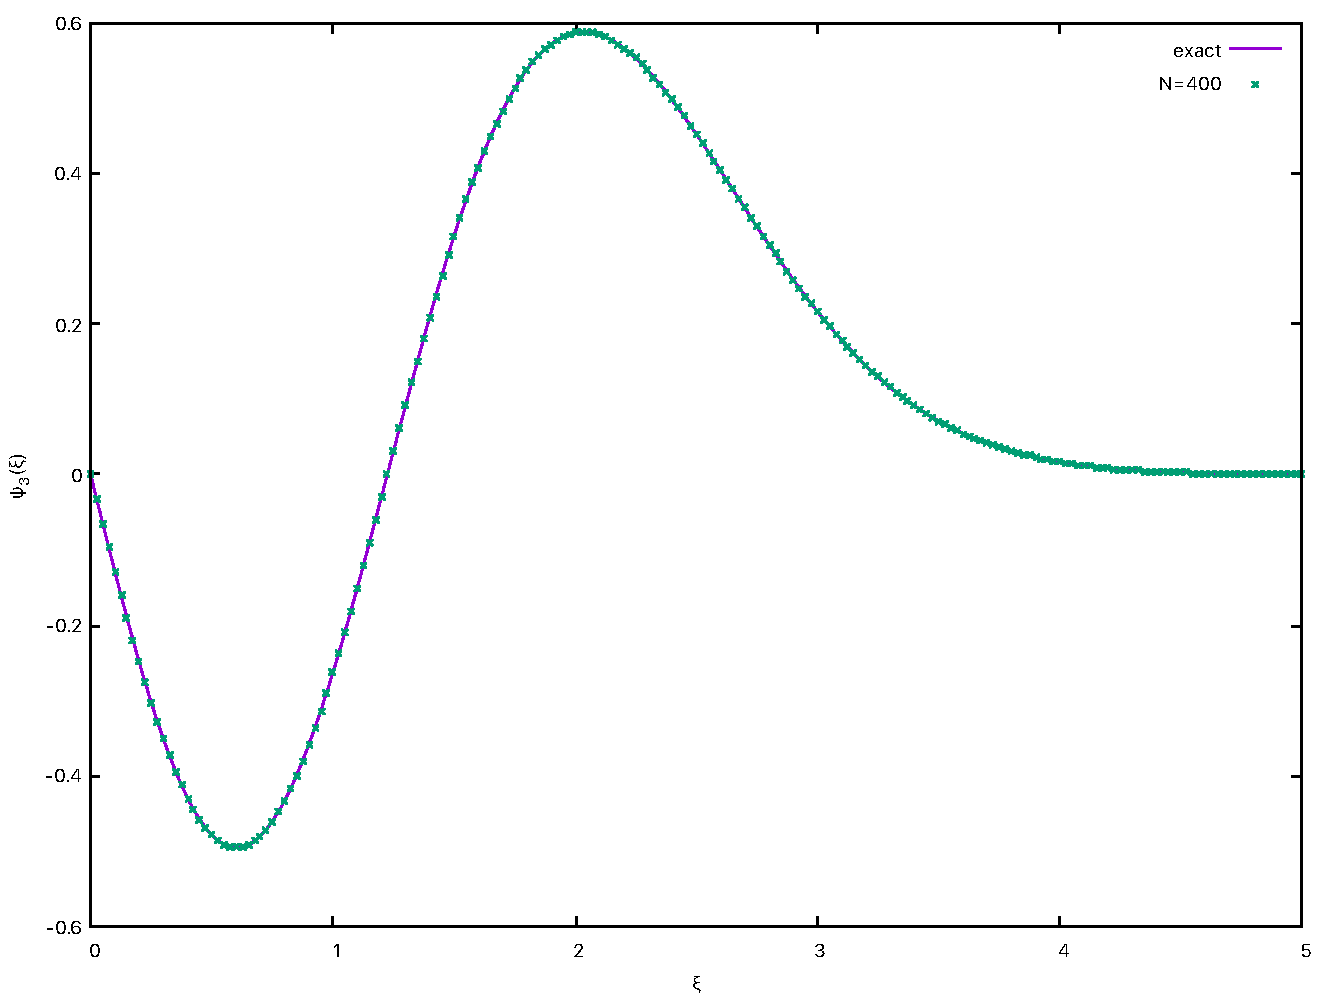
\includegraphics[width=0.75\linewidth]{../gnuplot/imageA.pdf}
\end{figure}
\end{frame}

% frame 21
\begin{frame}{Probability Density}
The following plot shows the quantum probability density as the square modulus of the computed wave function. The classical inversion points are obtained as:
$$V(\xi_{cl})=\frac{\xi_{cl}^2}{2}=\varepsilon_n=n+\frac{1}{2}\text{, so }\xi_{cl}=\pm\sqrt{2n+1}.$$
For $n=3$, outside $[-\sqrt{7}\approx-2.65,+\sqrt{7}\approx+2.65]$, the quantum probability decays \textbf{exponentially}.\\
\vspace{\baselineskip}
Classical probability density is instead defined only inside the above interval and diverges at $\xi_{cl}$ as:
$$\rho(\xi)\propto\frac{1}{\sqrt{\varepsilon_n-\xi^2/2}}.$$
\end{frame}

% frame 22
\begin{frame}{Comparison}
Quantum and classical probability densities, shifted by the eigenvalue $\varepsilon_3$, are plotted together with the potential $V(\xi)$.
\begin{figure}
\centering
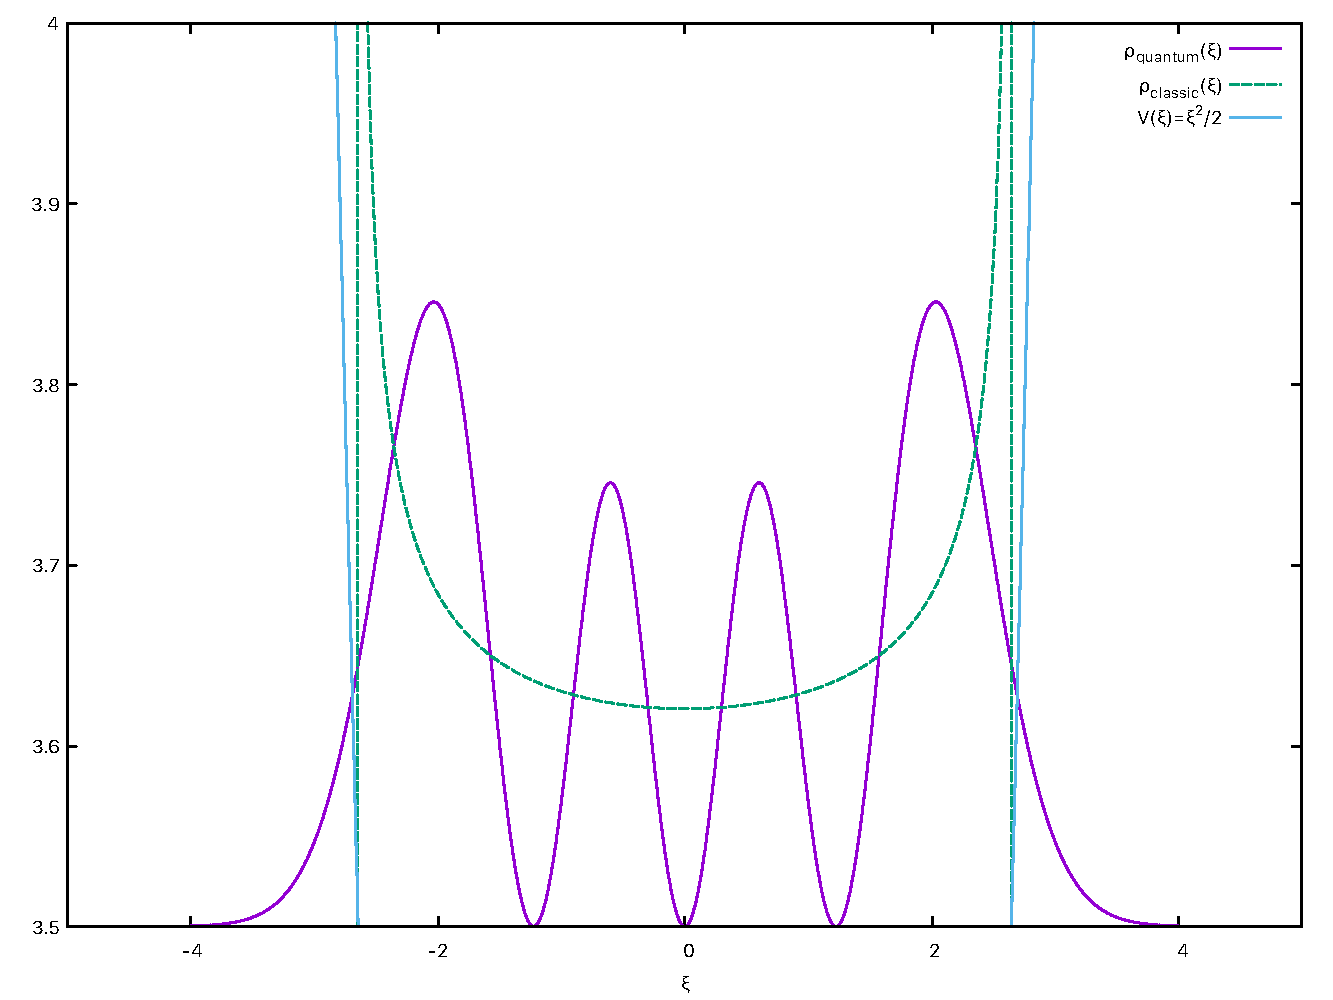
\includegraphics[width=0.75\linewidth]{../gnuplot/imageB.pdf}
\end{figure}
\end{frame}

% frame 23
\begin{frame}{Global Error}
The absolute value \textbf{difference} between the exact eigenvalue and the computed energy is taken as a measure of global error:
$$E(\Delta \xi)=|\varepsilon_n-\varepsilon_{computed}(\Delta \xi)|.$$
As discussed in general for Numerov's method, this is expected to go to zero no faster than $\Delta\xi^4$. An estimate of this order of convergence is given by:
$$p=\lim_{\Delta \xi\to 0^+}\log_2\frac{E(\Delta \xi)-E(\Delta \xi/2)}{E(\Delta \xi/2)-E(\Delta \xi/4)}.$$
For the three values of $\Delta \xi\in\{10/1600,10/800,10/400\}$, the above expression results $p\approx2.96$.
\end{frame}

% frame 24
\begin{frame}{Error Order}
Also this plot confirms that the order of the error is $O(\Delta \xi^3)$, instead of the lower \textbf{bound} $O(\Delta \xi^4)$.
\begin{figure}
\centering
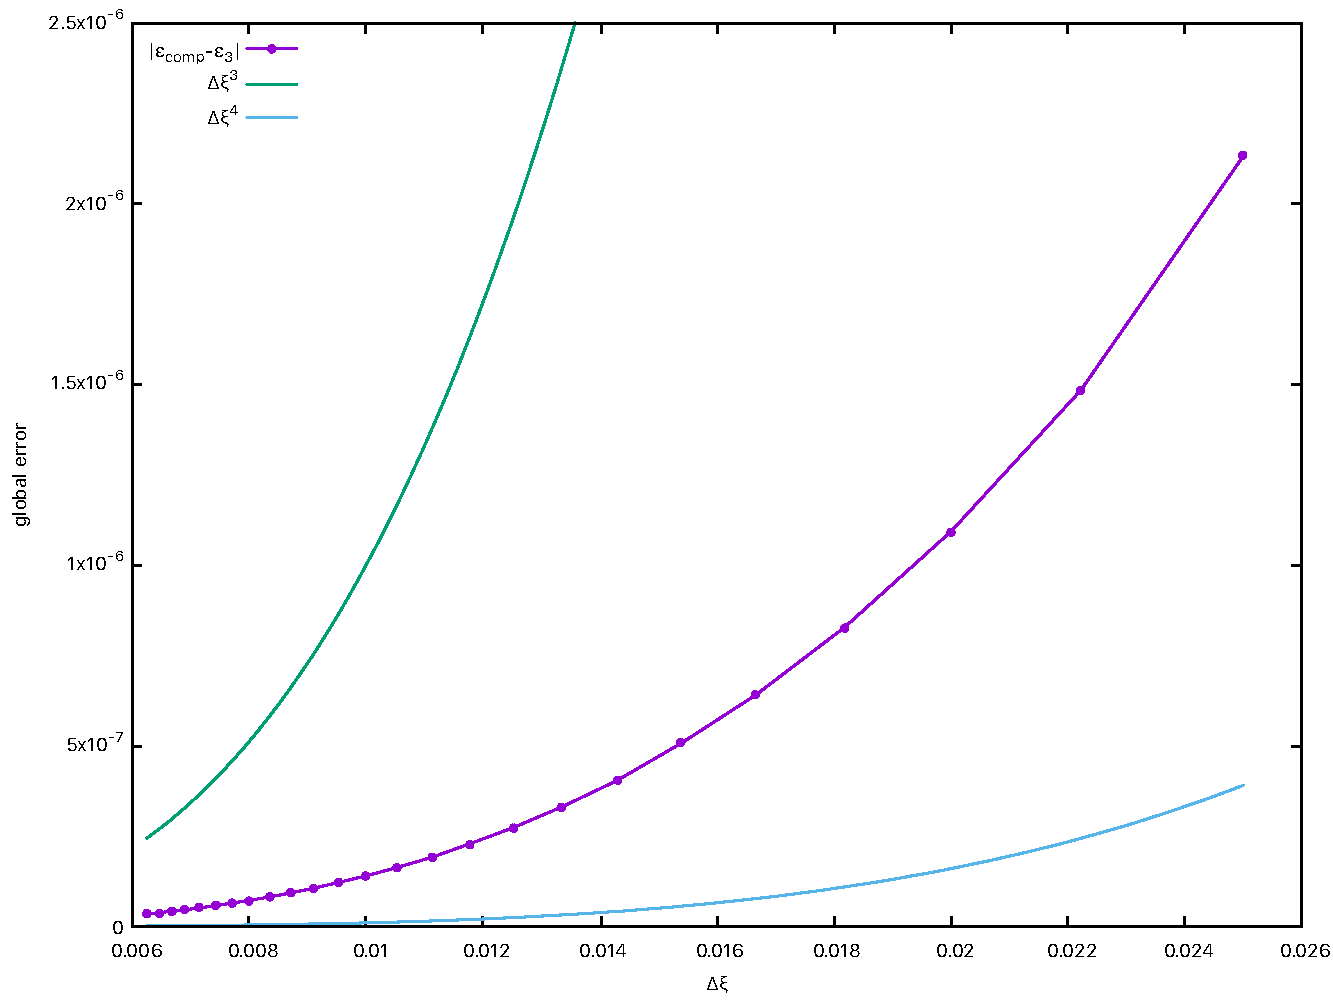
\includegraphics[width=0.75\linewidth]{../gnuplot/image3.pdf}
\end{figure}
\end{frame}

% frame 25
\begin{frame}{Lower Order}
The reason behind a performance worse than the lower bound of Numerov's method is that, somewhere in the code, a lower order error is introduced.\\
\vspace{0.5em}
If the expansion of $y_i^{L}$ and $y_i^{R}$ around $y_i$ is truncated to the second instead of the third order, the derivative discontinuity is evaluated as:\vspace{0.5em}
$$y_i'^R-y_i'^L=\frac{y_{i+1}^R+y_{i-1}^L-2y_i}{\Delta \xi}+O(\Delta \xi).$$
\vspace{0.5em}
\\This estimate is one order of error \textbf{worse} than the previous one. The following plot shows that one order of convergence is lost using this estimate.
\end{frame}

% frame 26
\begin{frame}{Slower Convergence}
Since the overall scaling gets worse, it means that the above poor estimate becomes the new \textbf{bottleneck} of the algorithm.
\begin{figure}
\centering
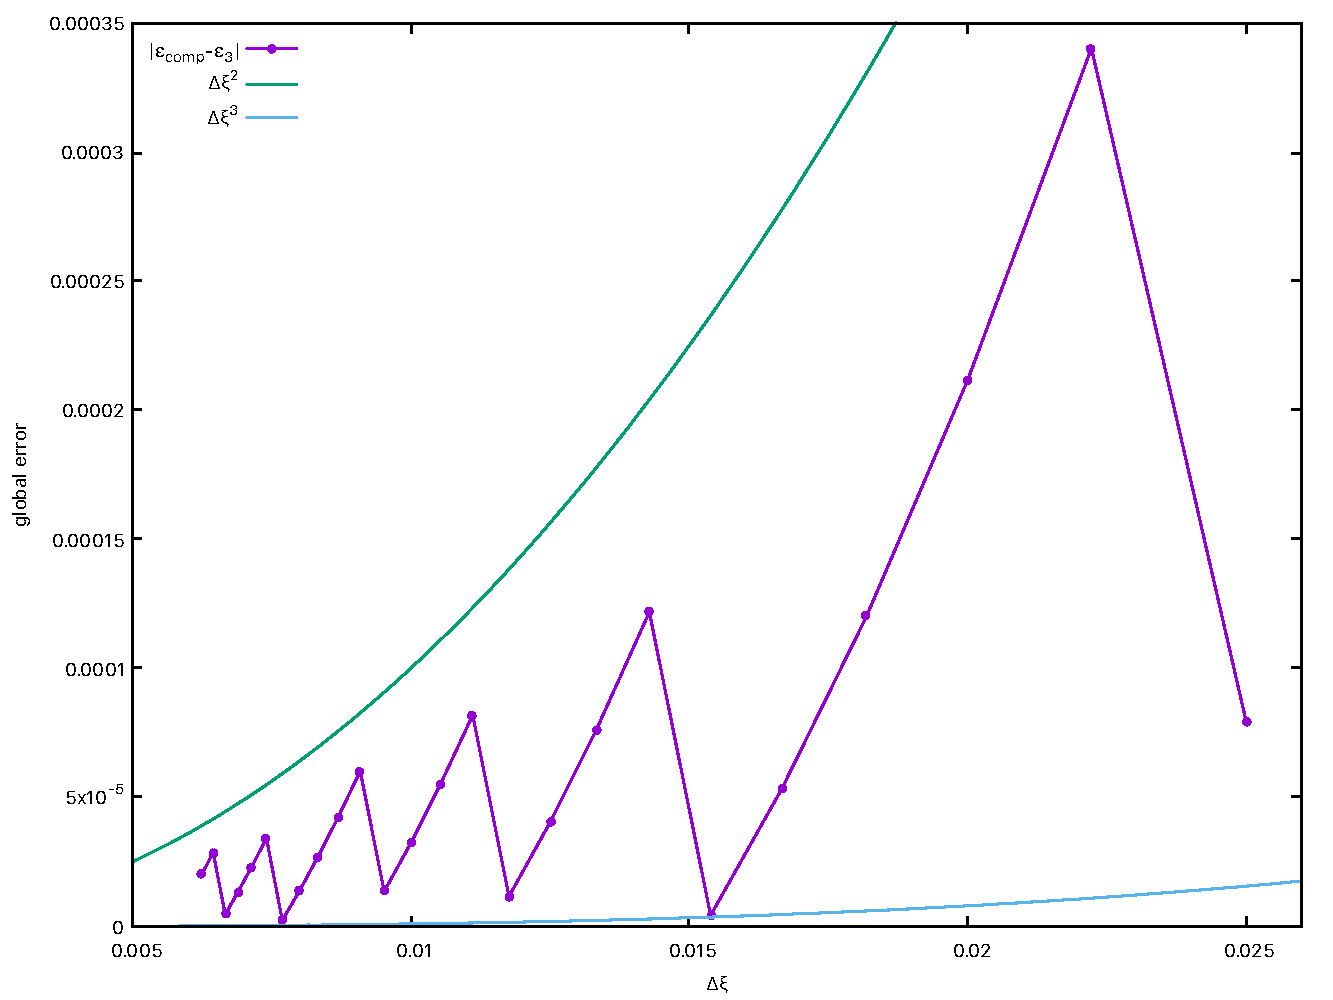
\includegraphics[width=0.75\linewidth]{../gnuplot/image2.pdf}
\end{figure}
\end{frame}

% frame 27
\begin{frame}{Higher Order}
If the expansion of $y_i^{L}$ and $y_i^{R}$ around $y_i$ is truncated instead to the fourth order, with the purpose of getting a more accurate estimate, the derivative discontinuity is evaluated as:
\vspace{0.5em}
$$y_i'^R-y_i'^L=\frac{y_{i+1}^R+y_{i-1}^L-(14-12f_i)y_i}{\Delta \xi(3-2f_i)}+O(\Delta \xi^3),$$
\vspace{0.5em}
\\since $y_{i}^{'''R}-y_{i}^{'''L}=-g_i(y_{i}^{'R}-y_{i}^{'L})$, as derived from the Schr\"{o}dinger equation of the harmonic oscillator.\\
\vspace{0.5em}
The fact that \textbf{no} global error improvement is found means that the bottleneck, preventing obtaining Numerov's order of error of $O(\Delta \xi^4)$, is not due to the derivative discontinuity estimate.
\end{frame}

% frame 28
\begin{frame}{Cusp}
Let again $i$ be such that $\xi_{cl}=i\Delta \xi$ and let $y_i$ be the prediction obtained using forward Numerov's formula centered in $y_{i-1}$.\\
\vspace{0.5em}
After backward integrating and matching, the issue is that Numerov's prediction for $y_i$, centered in the same $y_i$, generally differs from $y_i$:
$$y_{cusp}=\frac{y_{i+1}f_{i+1}+y_{i-1}f_{i-1}+10f_iy_i}{12}\neq y_i.$$
\\ This inexact result is the exact one of \textbf{another} problem, in which a Dirac delta function $v \delta (\xi-\xi_{cl})$ is superimposed at $\xi_{cl}$.\\ \vspace{0.5em} For the same argument of derivate continuity, a diverging potential produces a derivative discontinuity: a cusp.
\end{frame}

% frame 29
\begin{frame}{Dirac Delta Coefficient}
To get coherent results from Numerov's formula also in $y_i$, it must be allowed to have $f_{cusp}\neq f_i$ since:
$$y_{cusp}f_{cusp}=y_if_i\text{ so }\delta f = f_{cusp}-f_i= f_i\bigg(\frac{y_i}{y_{cusp}}-1\bigg).$$
Differentiating $g(\xi)=-2(\varepsilon-V(\xi))$, it follows that $\delta g=2\delta V$ and from the definition of $f(\xi)$, it is that $\delta g = 12\delta f/\Delta \xi^2$. Therefore:
$$\delta V = \delta f \frac{6}{\Delta \xi^2}=v.$$
Then, the above estimate of $\delta f$ allows to compute the \textbf{coefficient} $v$ of the Dirac delta function centered in $\xi_{cl}$.
\end{frame}

% frame 30
\begin{frame}{Perturbation Theory}
The first order \textbf{correction} to the energy eigenvalue $\varepsilon_n$ is given by the expectation value of $\delta H=\delta V\delta(\xi-\xi_{cl})$, the perturbation Hamiltonian, on the unperturbed eigenstate $\psi_n$:
$$\delta \varepsilon_n = \expval{\delta H}{\psi_n}=\int\delta f\frac{6}{\Delta \xi^2} \delta (\xi-\xi_{cl})|\psi_n|^2d\xi.$$
The integral is written as a sum on the grid and its only non-zero contribution comes from the interval of width $\Delta \xi$ around $\xi_{cl}$, so:
$$\delta\varepsilon_n=\delta f\frac{6}{\Delta \xi}|y_i|^2.$$
This first order estimate of the difference between the eigenvalue of the inexact problem and $\varepsilon_n$ is used to adjust the trial energy $\varepsilon$.
\end{frame}

% frame 31
\begin{frame}{Error Order Improvement}
A tolerance is set also on $|\delta \varepsilon_n|$. With this adjustment, the algorithm reaches Numerov's method error order lower bound of $O(\Delta \xi^4)$.
\begin{figure}
\centering
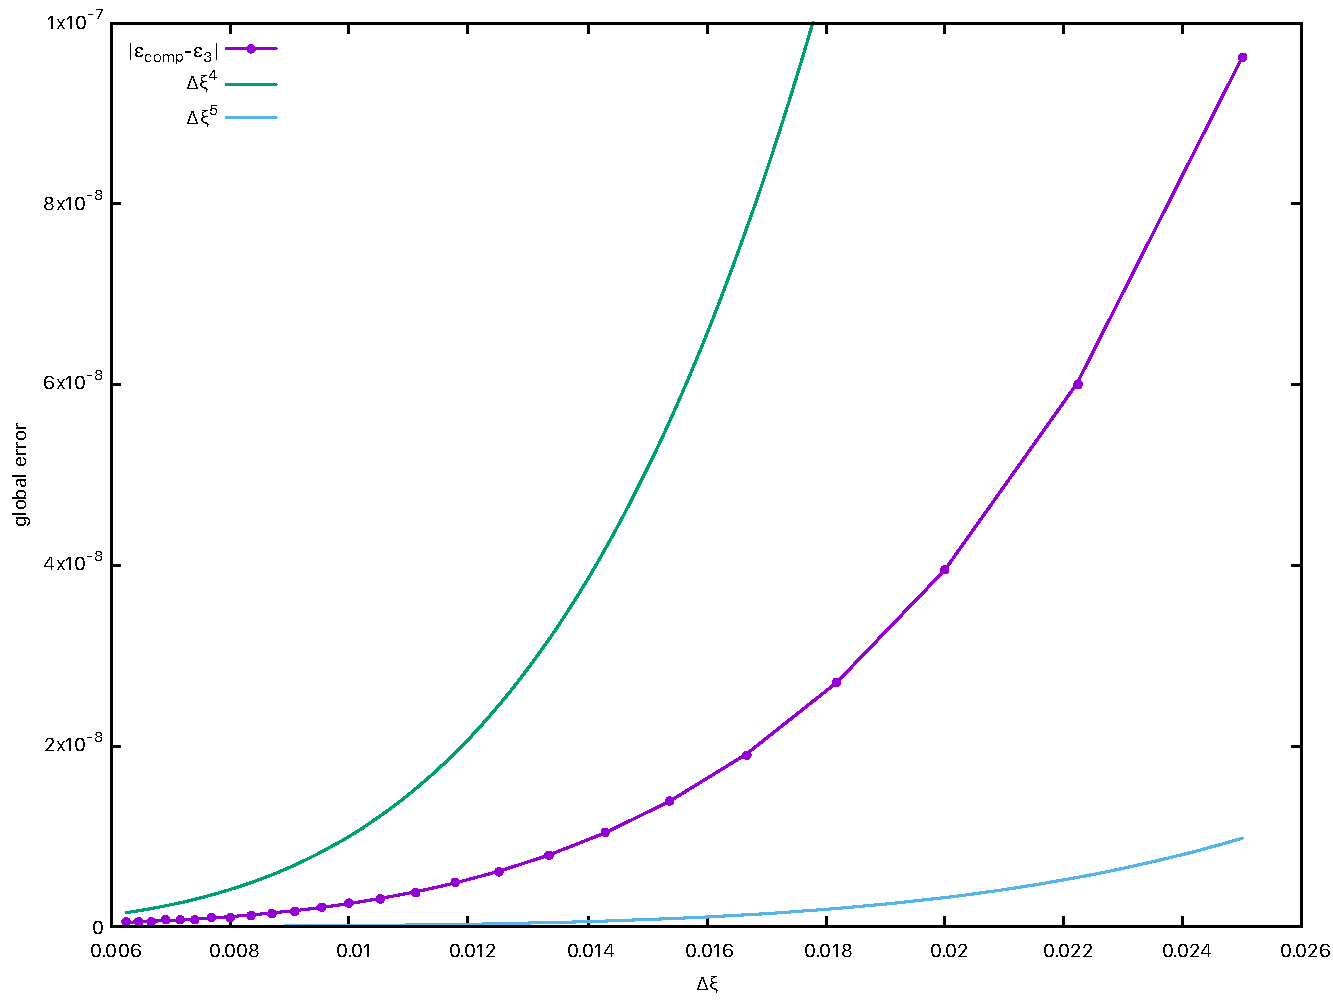
\includegraphics[width=0.75\linewidth]{../gnuplot/image5.pdf}
\end{figure}
\end{frame}

% frame 32
\begin{frame}{Conclusion}
The threshold on the size of $|\delta \varepsilon_n|$ substitutes the previous one on the width of the $[\varepsilon_{\min},\varepsilon_{\max}]$ interval, so both are set to $10^{-10}$ in units of $\hbar\omega$.\\
\vspace{\baselineskip}
For the same three values of $\Delta \xi\in\{10/1600,10/800,10/400\}$, the order error estimate correctly results $p\approx4.00$.\\
\vspace{0.5em}
\begin{itemize}
\item The above result shows that the bottleneck in the original code was in the process of halving the energy interval while backward integrating and looking for the eigenvalue $\varepsilon_n$.\\
\vspace{0.5em}
\item The code reaches now the error order lower \textbf{bound} admitted using Numerov's integration method and no further improvement can be obtained using this algorithm.
\end{itemize}
\end{frame}

\end{document}